\chapter{Crisis situation models that serve social media operators}

\section*{Introduction}
The context presented in the literature review highlighted the importance of the management of information during an emergency events.
Improving the response requires better coordination between the different actors.
However, a coordinated response can only be performed if all the partners easily share information.
The first chapter used the example of the Common Operational Picture (COP) as a visual medium for information sharing.
The COP makes it possible to display certain information with a vocabulary common to all actors.
However, this approach requires that all the actors agree beforehand on the information of interest.
During the preparation phase, COP are a ways to create common situational understanding between the different actors \parencite{steen-tveitCommonOperationalPicture2021}.
Also, the integration of information obtained from social media into this interface remain a challenge.
The previous chapter identified three aspects that could use a better information input using social media data:

\begin{itemize}
    \item Collaboration: the need for information to support coordination between partners
    \item Situational awareness: the need for information that enables the identification of the elements that make up the environment
    \item Public communication: the need for information to understand the population's feelings regarding the event and facilitate public relations.
\end{itemize}

These needs are directly linked with the first sub-problem consecutive to the primary research question, namely: \emph{What is information obtained from social media relevant to decision-makers in crisis response?}
This chapter seeks to identify this relevant information to be able to collect it automatically later on.
The information must therefore both meet the need for information, but also be able to be manipulated by a computer.
As a result, the approach is twofold.
A first section reviews the previous studies on the information manipulated by the actors of the crisis.
This section is then based on the literature and meetings with crisis management practitioners.
The second section focuses on the previous models of crisis situations proposed.
These crisis situation models consist of abstract, but automatable, representations of the information used for crisis management.
Finally, a third and last section crosses the needs identified by the two previous sections.
It presents the information that can be automatically retrieved to support decision making.
This is the same information that the following chapter seeks to recover.

\section{Information expected by practitioners}
This chapter thus draws on the results of previous research and works realized alongside social studies conducted during the PhD by social scientists.
This section is split in three parts.
The first part zoom on the processing of social media in crisis management organization.
It aims at answering the question \textit{Who is processing social media content in these organizations?}
A second part focuses on the information already identified in the literature.
Finally, the last part merge both worlds and present a first set of information that enable decision-making.

\subsection{Social media processing in crisis management organizations}
Crisis management organizations are composed of several actors with well-defined roles.
As the first chapter mentioned, crisis management involve multiple actors and not all of them are paying attention to social media content.
While decision-makers benefit from the insights coming from these platforms, they do not perform the collection themselves.
This section reports on the place of social media in different organizations observed in the course of this work.
The research question that this part aims to answer is:
\blockquote{RQ: Who is in charge of social media handling in crisis response organizations?}
The observations and interviews with practitioners, associated with previous results from the literature, contribute to answer the two previous RQs.

\subsubsection{Method}
The diversity of actors involved in this PhD, as well as the France-U.S. distribution, allowed to meet and exchange with a wide variety of actors.
This variety is all the more welcome since, as presented in the next section, the treatment of social media in management knows no standard.
At least five occasions (summarized Table~\ref{table:terrain-summary}) provided valuable insights in the scope of the study.

\begin{table}[hbp]
    \centering
    \caption{Overview of the different meetings with practitioners.}
    \begin{tabular}{m{0.25\textwidth} m{0.6\textwidth} m{0.15\textwidth}}
        Occasion (Location)                    & Participants profiles                                                                                                                                          & Methodology          \\ [0.5ex]
        \toprule
        PSAPs Role Play (Charleston, SC)       & Call takers, Dispatchers                                                                                                                                       & Role-plays           \\
        Early Adopters summit (Charleston, SC) & 25 local 911 professionals (PSAPs Managers, Call-takers, Dispatchers and IT technicians)                                                                       & Focus groups         \\
        Exercice 1 MACIV (Dpt, Var)            & Professional and volunteer firefighters                                                                                                                        & Exercise Observation \\
        Exercice 2 MACIV (Dpt, Vienne)         & The staff of the Prefecture 86, a communication officer, two representatives of the police, firefighters and gendarmerie                                       & Exercise Observation \\
        Exercice 3 MACIV (SW Zone)             & South-West Zone and six of the twelve associated Préfectures (the 79, 47, 40, 17 ,23, 87). The Préfectures had a similar composition as the one in exercice 2. & Exercise Observation \\
        \bottomrule
    \end{tabular}
    \label{table:terrain-summary}
\end{table}
a person in charge of communication, two representatives of the police, the fire department, the gendarmerie and other services (cartography, road infrastructures, etc.).

% * Roleplay
In the U.S., \textcite{graceRolePlayingNext2019} conducted role-plays at the Public-Safety Answering Point (PSAP) of Charleston (South Carolina).
This PSAP is tasked with answering calls from citizens and dispatching resources during emergency situations.
The particularity of this PSAP is its adoption of a system allowing it to consider
text messages (SMS) and reports from Internet platforms (social media) in addition to calls.
One of the objective of these role-plays was to define with the call-takers and dispatchers what a perfect social media could be for them \parencite{kropczynskiIdentifyingActionableInformation2018}.
The study in the U.S. took place in the context of the development of Next-Generation 911.
As per the authors:
\blockquote{Next-Generation 911 (NG911) infrastructure will replace analog systems
    designed to support voice services for landline 911 callers with digital, IP-based systems that
    will allow smartphone users to “call” 911 via voice, text, image, and streaming video.}
The objective of these role-plays was to document how call center operators processed the information that came to them from calls.
The inten and how this could be reflected in social media.
This exercise highlighted many aspects of call center operations.
First of all, there are two types of operators who interact with information: call-takers and dispatchers.
Call-takers are responsible for receiving calls and getting the right information from the callers.
The answers are shared with the dispatchers through the Computer-Aided Dispatch (CAD).
The CAD system allows for the entry of notes associated with the call.
The call-takers teams also use a CAD plugin called ProQA.
ProQA is an integrated expert system that provides a support function through question proposals and classifications for the event.
Protocols, as interpretive frameworks, shape information gathering and filtering.
The information pipeline in the case of the PSAPs was the following:

\begin{enumerate}
    \item A \textit{Caller} calls the PSAP through the 911
    \item The \textit{Call-taker} receives the phone call, asks questions to the caller to obtain as much information as possible about the event.
          They then record their findings on the CAD system.
    \item The \textit{Dispatchers} receive an alert from the CAD that a new event is in progress. They then consult the notes provided by the call-takers to dispath resources.
    \item The \textit{Responders} follow the instructions provided by the dispatcher to intervene on the scene of the incident.
\end{enumerate}

% * Early adopters summit
The 2019 911 Early Adopters’ Summit provided the opportunity to meet 911 practitioners on the topic of NG911.
This summit was composed of many different profiles: managers of PSAPs, but also call-takers, dispatchers and IT technicians.
The participants met during this event, as early adopters, were largely in favor of changes in emergency response.
\textcite{graceCommunicatingNextGeneration9112020} reports their feelings and opinions through a Strenghts-Opportunities-Weaknesses-Threats (SWOT) analysis \parencite{gaoConsolidatingSWOTAnalysis2011} on NG911.
The SWOT analysis last an afternoon an implied 25 participants, all of them being 911 professionals.
This type of analysis allows to identify strenghts and weaknesses (internal or external) of an organization.
The goal was then to reflect on these factors in the case of NG911 through the lens of this method.
The summit was also the occasion to capture the diversity of configurations of PSAPs that exist in the US.
Indeed, the setup documented during the Charleston role-plays is not standard, and each PSAP center is free to organize as it prefers.
So, depending on the constraints applied to the center, its structural organization might different.
The call center can report to a remote dispatch center, along other call centers for instance.

% * Exercices MACIV
In France, the MACIV exercises were opportunities to observe how professionals respond in practice to a situation.
Figure~\ref{information:french-orga} illustrates the organization of the institutions in charge of the crisis response.
It is a hierarchical organization.
The hierarchy is based on the size of the area affected by the event.
The higher layer is the National level (not represented in the figure), then the Zonal level, the Départemental level and the Communal level.

\begin{figure}[htb]
    \centering
    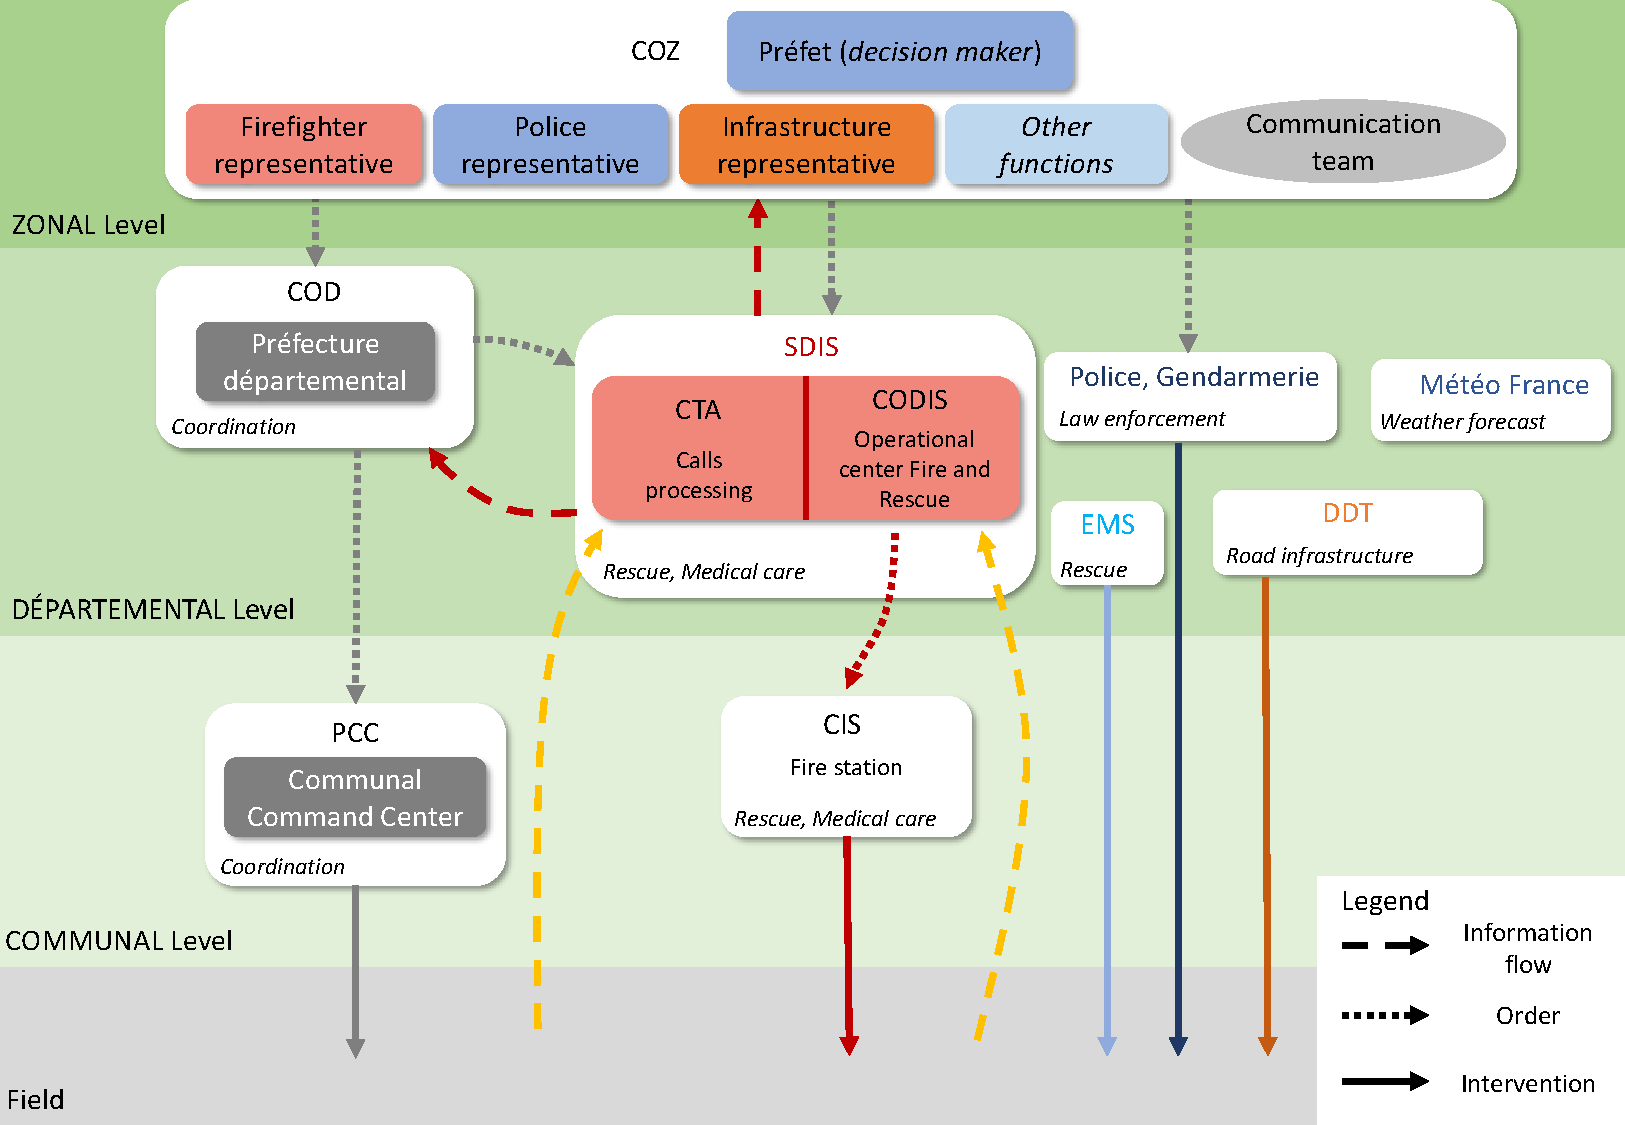
\includegraphics[width=\textwidth]{figures/chap-3/orga-gestion-crise.pdf}
    \caption{Diagram of the organization of the different French institutions involved during the response to an event of zonal scale. Illustration adapted from \textcite{batardIntegrerContributionsCitoyennes2021}}
    \label{information:french-orga}
\end{figure}

The Zonal and Départemental levels are governed by Préfectures (administratives institutions in charge of representing the government authority).
The services in charge of crisis response in these institutions are respectively the Centre Opérationnel de Zone (COZ) and the Centre Opérationnel Départemental (COD).
The Départemental level also includes the highest levels of representation of the response actors (firefighters, police, emergency services, etc.).
Among them, the Service Départemental d'Incendie et de Secours (SDIS, for \textit{Departmental Fire and Rescue Service}) is in charge of managing the rescue teams according to the priorities fixed by the COD.
The SDIS serves two function: i) organized the rescue units and ii) handle phone calls.
The calls are handled through the Centre de Traitement des Appels (CTA, for \textit{Calls Processing Center}).
The organization and management of rescue teams is performed by the Centre Opérationnel Départemental d’Incendie et de Secours (CODIS).
The Centre Opérationnel de Zone provides instructions to the Centre Opérationnel Départemental or directly to the SDIS (see definition below).
The SDIS takes its orders from either the COZ or the COD.
It provides orders directly to the commanders of the unites deployed or officiers in charge of sub-centers—the CIS.
It receives back reports from the rescue teams and phone calls from victims.
They provide the information they have to the COZ and COD.
The last actor is the PCC and is the crisis cell created in each Commune (equivalent of Counties).

Another important player in these exercises was the VISOV association.
The Volontaires Internationaux en Soutien Opérationnel Virtuel (VISOV, french equivalent of the \textit{Virtual Operations Support Teams} — VOST) association is of volunteers.
These citizens organize themselves to help the institutional actors to identify the information related to an event posted on the social media.
Their organization is further developed in \textcite[p.122--148]{batardIntegrerContributionsCitoyennes2021}.

The exercises involved three types of actors: an institutional actor, an association of volunteer citizens and the research teams.
These exercises took place in the following manner.
First of all, a preparation of the exercise (role of each actor, choice of the type of crisis, actors involved according to their availability, etc.)
Then comes the exercise itself.
During the exercise, the institutional actors play their roles and respond to the event as they would normally do.
The VISOVs support the insitutionals by processing the social media content provided for the exercise.
Finally, the research teams shadow the practitioners in their roles.
At the end of the exercise, an exchange phase allows the participants to give feedback on the exercise.
The main purpose of these exercises was to document the information flow within the French emergency management institutions, and particularly, the way information coming from social media were considered.
The types of events simulated were, respectively:

\begin{itemize}
    \item Flooding event in the Var Department at the Service Départemental d’Incendie et de Secours du Var (SDIS83).
    \item Snow event and consecutive traffic jam in the Vienne Department at the Vienne's Préfecture.
    \item Chemical incident in the South West of France involving the South-West Zone and six of the twelve associated Préfectures (the 79, 47, 40, 17 ,23, 87) and the CODIS 47.
\end{itemize}

% ? Premier exercice
The three exercises were an opportunity to observe different institutions and the way they approach social media.
In the first exercise, social media were processed inside the SDIS83\footnote{each french Department is associated with a number. In this case, the Var Department has the number 83}
by a Médias Sociaux en Gestion d’Urgence operator (MSGU, french equivalent of the \textit{Social Media in Emergency Management} — SMEM).
The setting of the SDIS is shown in Figure~\ref{information:exercice-1-setup}.
The decision maker was a firefighter officer, in charge of the room.
The officier was assisted by four firefighters that were managing the teams dispatched and their reports using a white board.
One of the firefighter was taking phone calls from victims.
Directly to his right was a volunteer firefighter trained to gather social media information during the event.
Behind these two operators was another specilized volunteer firefighter was in charge of the cartographic desk.

\begin{figure}[htb]
    \centering
    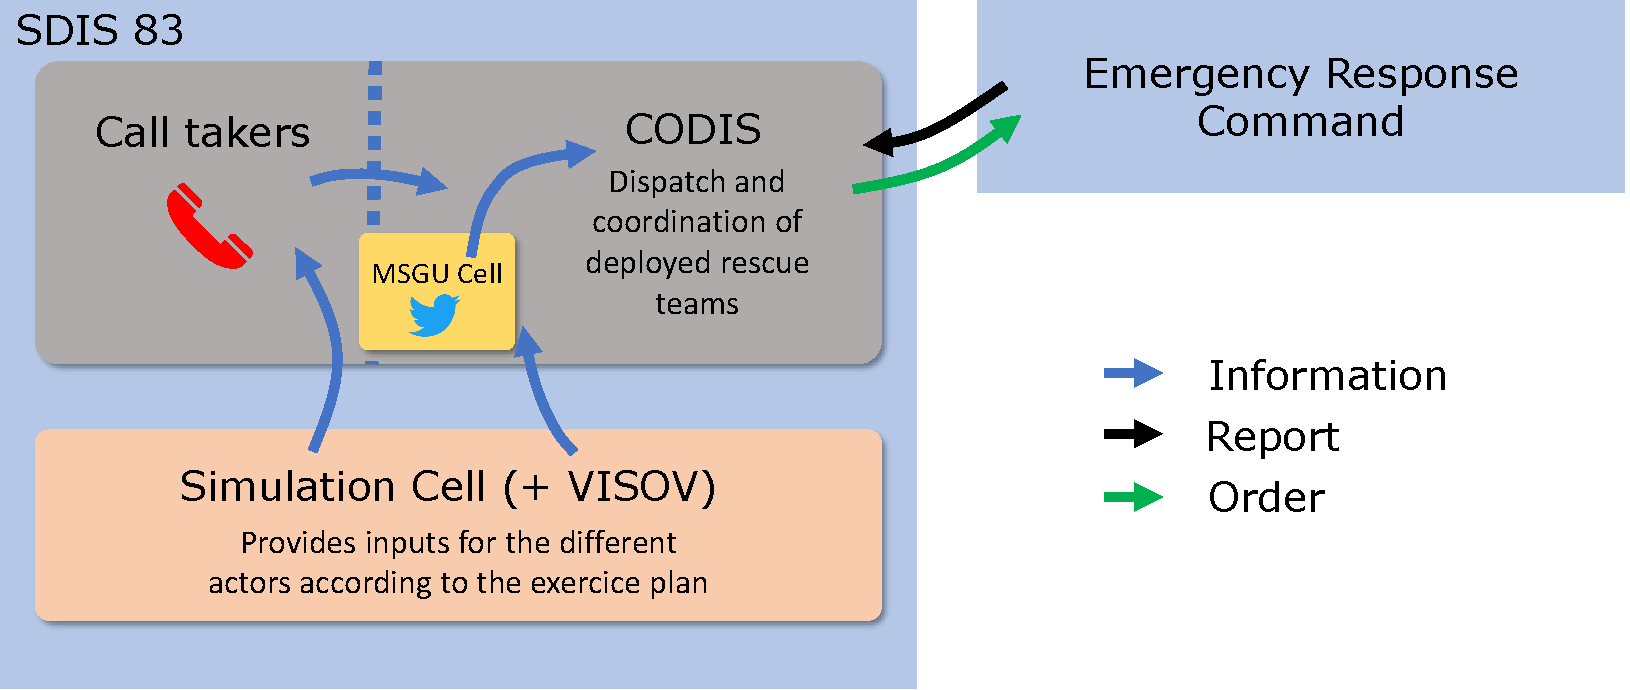
\includegraphics[width=\textwidth]{figures/chap-3/exercice-1-setup.pdf}
    \caption{Organizational diagram of Exercise 1 MACIV at SDIS83 in the Var Department. Illustration adapted from \textcite{batardIntegrerContributionsCitoyennes2021}.}
    \label{information:exercice-1-setup}
\end{figure}

The social media operator was who is familiar with social media and communication.
This operator was sharing a Google Sheet\footnote{https://www.google.fr/intl/fr/sheets/about/} document with the members of the VISOV association.
A Google Sheet document is a tabular file identic to an Excel file, where multiple persons can modify simultaneously the document and see the changes in real time.
It is the possibility of having several actors collaborate in real time on the same document that motivated the choice of this format.
The VISOV association is mostly composed of volunteers with a background in public service, rescue operations etc.
These volunteers monitor social media on their own to identify information related to a potential, or already ongoing event.
This operator was monitoring social media and cross-referencing the information they could obtain with that provided by the VISOV volunteers.
This live document is then shared with the person in charge of social media processing within official institutions.
Using their own findings and the ones from the online document, the MSGU operator will then provide the information obtained when asked by the decision-maker in the room.

% ? Deuxième exercice
The second exercise, took place in the Vienne département at the 86 Préfecture in the city of Poitiers.
The institution studied was the Prefecture of Vienne through their COD and their communication cell Figure~\ref{information:exercice-2-setup}.
The COD was composed of a decision-maker (played by a subordinate of the Prefect), a person in charge of communication, two representatives of the police, the fire department, the gendarmerie and other services (cartography, road infrastructures, etc.).
This institution uses a software similar to the CAD software used in the U.S. to share information.
This information system is called SYNERGI (SYstème Numérique d’Échange, de Remontée et de Gestion des Informations).
The Prefecture did not have a dedicated social media handling service (MSGU) as in the first exercise.
Instead, the VISOV association transmitted their findings directly to the communication unit.
In this configure, the institution was more reliant on the processing realized by the VISOV association.
The operators in charge of the social media in the Préfectures were persons from the communication team of each Préfecture.
In this case, these persons were not familiar with emergency or rescue operations.
They were mostly tasked with communication to the public using the official accounts of the institution they were part of.
Monitoring of social media activity and information gathering were not the priorities of these operators.

\begin{figure}[htb]
    \centering
    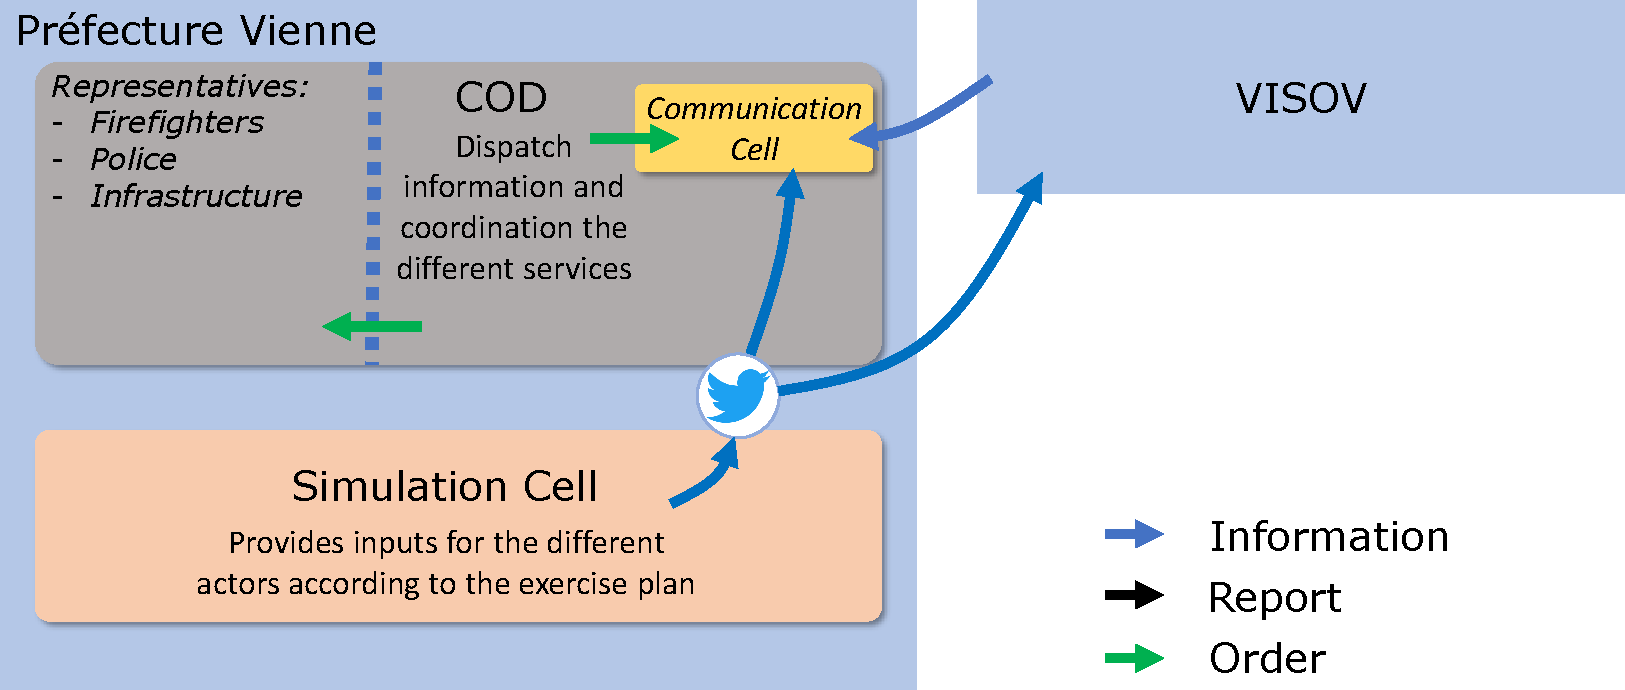
\includegraphics[width=\textwidth]{figures/chap-3/exercice-2-setup.pdf}
    \caption{Organizational diagram of Exercise 2 MACIV at the COD in the Vienne Department. Illustration adapted from \textcite{batardIntegrerContributionsCitoyennes2021}.}
    \label{information:exercice-2-setup}
\end{figure}

% ? Troisième exercice
The third exercise, saw similar actors involved but at a bigger scale.
Instead of one Préfecture, six were present under the direction of a Préfecture Zonal (see Figure~\ref{information:french-orga}).
The setting of this exercise is illustrated in Figure~\ref{information:exercice-3-setup}.
Each Préfecture involved the same organization as the one in the second exercice (rescue team representatives, communication cell, speciallized functions).
ALso in this exercice, there was no MSGU created by the institutions.
As a result, they also relied on the VISOV association to obtain information from social media.
Also the participating Préfectures were using the SYNERGI to exchange official information.

\begin{figure}[htb]
    \centering
    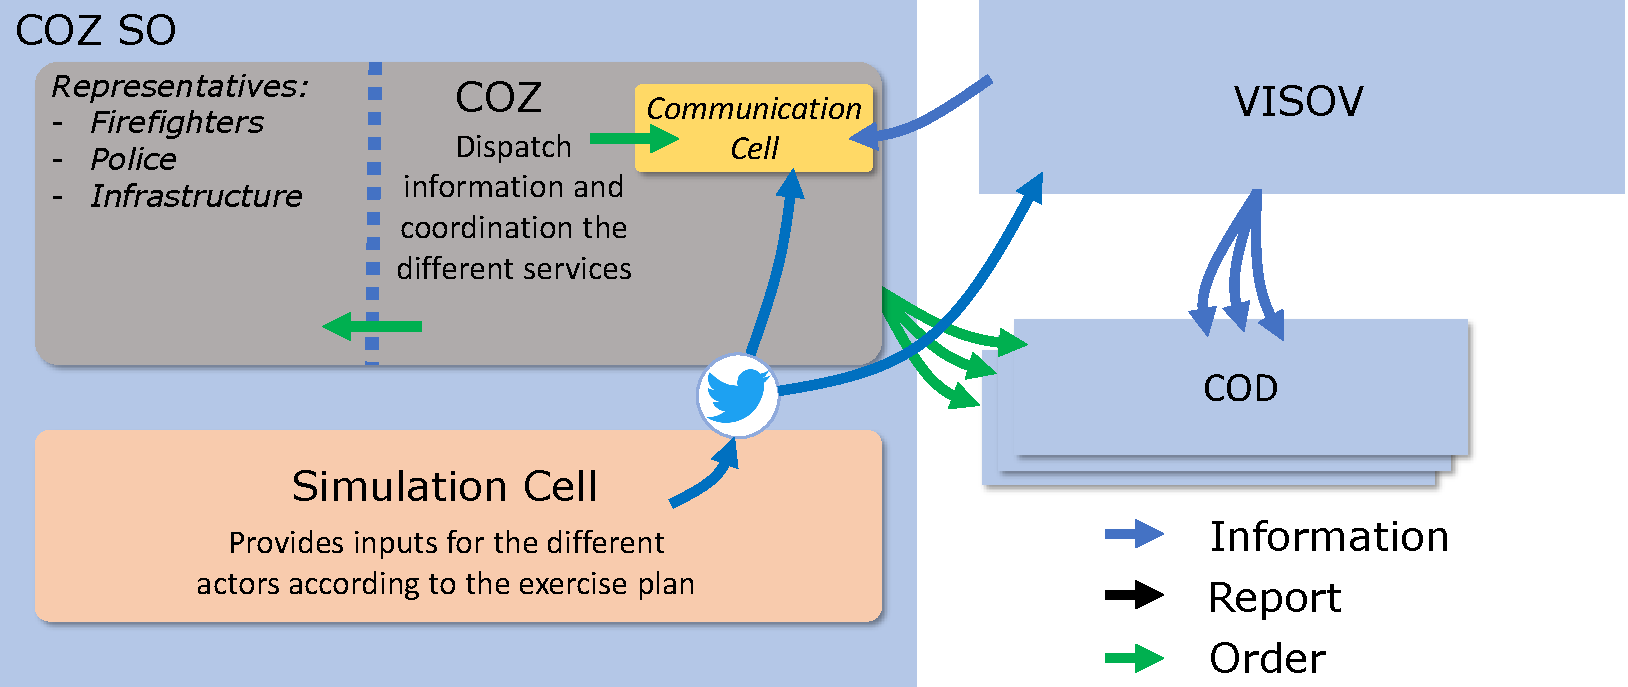
\includegraphics[width=\textwidth]{figures/chap-3/exercice-3-setup.pdf}
    \caption{Organizational diagram of Exercise 3 MACIV in the different Préfectures involved. Illustration adapted from \textcite{batardIntegrerContributionsCitoyennes2021}.}
    \label{information:exercice-3-setup}
\end{figure}

\subsubsection{Findings}
The various exchanges with the practitioners allowed us to better understand their functioning, their problems and their overall feeling on the issue of social media.
The opportunity to carry out these observations in two different countries also allows to better understand if some difficulties are local or shared between the two continents.
This section thus presents the key findings of these interviews.

\paragraph{A lack of tooling for processing social media content}
% * Done
The results of the SWOT analysis reveals that the participants particularly understood the value of this system.
Participants cite an improvement in the resilience of their information pipeline, thanks to the inclusion of new information channels such as social media that allow to cross-check the information obtained.
They also see NG911 as an opportunity to improve situational awareness of ongoing events .
On the other hand, participants noted concerns, mostly related to the digitalization of their work environment.
The volume, variety and speed of data provided by different platforms exposes PSAPs to numerous threats such as misinformation and cybercriminals.
Participants also mentioned privacy issues.
The above threats require new protocols and tools for processing and new training for the personnel assigned to these new tasks.
However, all these new features come at a price, and cost was identified as one of the main concerns about NG911.
Hence, social media processing systems, while they are wished by some practitioners, did not reach them yet.
Similarly, in France, the information system used in crisis response, SYNERGI, has some critics.
\textcite{linotPerspectiveComputationnelleDefi2018} report that the SYNERGI users' suffer from:

\begin{itemize}
    \item Its rigidity, which leads to system circumvention;
    \item Communication issues, caused by a lack of common vocabulary;
    \item The diversity of unprepared institutions involved, leading to poor coordination;
    \item Lack of context associated with the information shared, adding confusion.
\end{itemize}

Also, the SYNERGI system prevents the collection or sharing of social media information in this platform.
The widespread use of the system and its official status hinders any rapid iteration on it.
The only integration of social media in an institution in France was during the first exercice.
But the system used was not official and was more like a home-made design that met a practical need.
Thus, it appears that the early adopters are unfortunately not so much.
Rather, they are individuals convinced of the value of social media in crisis management.
However, due to the lack of tools offering the necessary capabilities, it is difficult to consider this technonology ready to enter the early adoption stage.
% Also, it is interesting to note the particular status of social media data within this information pipeline.
% \textcite{castagninoWhatCanWe2019} highlights the segregation of social media, systematically assumed as untrustworthy information during the first exercise.

\paragraph{Heterogeneous profiles of social media operators}
% * Done
The different sessions also allowed us to understand the diversity of profiles of people who deal with social media in crisis management.
The PSAPs encountered envisioned the role as an adaptation of call takers.
Thus, either an operator would be dedicated to social media monitoring, or existing call takers would be provided with an interface to monitor content of interest.
In the past, when VOSTs were still in operation, some PSAPs (notably in the Colorado State) used these volunteers to assist them.
This third party operation was found during the MACIV project exercises.
In France, media operators can be found at different levels in the hierarchy of response actors.
For the time being, this distribution depends on the interest that each one has in social media.
In the case of the first exercise, the SDIS had a dedicated operator alongside their call-taker and were cross-checking information.
In the other two exercises, it was the communication cell of the Prefectures that was monitoring social media, to provide information to the decision-makers.
In all French cases, their operators were assisted by a third-party of volunteers, VISOV.
Overall, the processing of social media in crisis cells is carried out in a relatively similar manner in France and the U.S.
Both countries dedicated a person to the processing, and keep this person in close proximity with the decision-makers.
For instance in France, the social media operator was in each exercice in the same room as the latter.
The organizations in charge of the response also rely (or have relied) on a partner (the VISOV in France or the VOST in the U.S.).
Conseqeuntly, the processing is not always directly made by the social media operator present in the crisis cell.
Thus, there is currently one or more intermediaries between the fact and the decision-maker, as may be the case with telephone calls or reports made by response teams.
Gathering information from social can then be challenging because of the current lack of framing in the process of information collection.
Finally, the skill profile of the operators is also currently very diverse.
In France, the profiles observed were those of communicators, while in the United States, the people considered would be specially trained.
In the former case, these profiles translate a vision more oriented toward information dissemination rather than information collection.
As reported in \textcite{castagninoWhatCanWe2019}, french emergency organizations systematically assume information coming from social media as untrustworthy information.
Thus, for them, social media is more a communication channel than a collection channel.

\paragraph{Framing information collection: the Six Ws}
\label{sec:sixws}
% * Done
The Role-Play session at the Charleston PSAP brought interesting in the way the information collection is framed by call-takers \parencite{kropczynskiIdentifyingActionableInformation2018}.
\blockquote{The “Six W’s”—Where, What, Weapons, Who, When, and Why—provide call-takers with
    a heuristic for questioning callers and entering only relevant information for each call.}
The call-takers from the 911 PSAP's frame their interviews with the callers through the Six W's.
The goal of the Six W's is to obtain information that match the information needs of the decision-makers.
These Six W's are:
\begin{itemize}
    \item \textit{Where} is the assistance needed,
    \item \textit{What} is the event taking place,
    \item \textit{Weapon(s)} involved in the event (if relevant to the nature of the event),
    \item \textit{Who} is involved in the event,
    \item \textit{When} the event started,
    \item \textit{Why} the event is happening.
\end{itemize}
These specific questions help the call-takers to acquire quickly specific information relevant for decision-making.
This information was previously identified as the most revelant information to respond quickly and effectively an emergency.

\subsection{A plurality of information needs in crisis management}
% TODO Checker cette partie
It appears that in the majority of cases, the information coming from social media passes through at least one intermediary before reaching the decision-maker.
Decision-makers need information, but they are not the persons actively monitoring social media.
Thus, the staff responsible for retrieving information from social media must therefore orient their research towards the needs of decision-makers.
Several questions therefore arise:

\begin{itemize}
    \item What information do decision-makers need?
    \item What information are the operators looking to retrieve?
\end{itemize}

The first question is at the heart of the crisis management system.
The decision-makers' needs have to be answered, and this is the role of the support operators (call-takers and social media operators) to fulfill these needs.
The second question looks at the information that operators search for in the stream of social media messages.
This question guides the development of the algorithms responsible for the retrieval of data presented in the next chapter.
The remainder of this section develops the analysis of this need in light of previous work that
has defined concepts such as situational awareness and actionable information.

\subsubsection{Situational awareness}
\label{sec:situational-awareness}
Situational awareness is summarized as the understanding of the "big picture" of a situation.
More precisely, it is the comprehension of the different aspects of an event, environment, and/or entities and how they are more likely to evolve in the near future.
Sufficient situational awareness is a critical factor in decision-making.
Each individual has their own situational awareness, depending on several factors such as experience, perception ability, training etc.
The group formed by individuals also carries its situational awareness.
As described in Chapter 1, emergency situations are confusing events that reset situational awareness.
The decision-makers in charge of the response must therefore build an updated mental representation of their environment.
This task is all the more difficult as the context is unstable and may continue to evolve as a result of aftershocks or cascade effects.
In addition, the amount of new information can be overwhelming, depending on the size or complexity of the event.
In the described context, it appears crucial that decision-makers rely on adapted methodologies and tools to reconstruct adequate situational awareness for decision-making.
This work and definition attracted the interest of the U.S. military, who embraced the concept, working permanently in a stressful and highly uncertain environment.
\textcite{departmentofthearmyAdvancedSituationalAwareness2021} compiles the doctrine they have built around the concept, including how it fits into the decision-making process and how situational awareness is influenced by the environment.

The currently dominant definition is seminal work presented in \parencite{endsleyTheorySituationAwareness1995}.
\citeauthor{endsleyTheorySituationAwareness1995}, propose a definition of situational awareness as well as a model to explain how it fits into the decision-making process.
They define situational awareness as the:
\blockquote{perception of the elements in the environment within a volume of time and space, the comprehension of their meaning and the projection of their status in the near future.}
This definition is associated with three levels: (1) perception, (2) comprehension, and (3) projection.
Perception refers to an operator's ability to detect relevant signals through its senses.
Level 2, comprehension, refers to the ability to interpret and make connections between the perceived signals.
Finally, level 3 corresponds to the ability to anticipate future events based on available information.
Figure~\ref{information:SA} provides an overview of situational awareness in the decision-making process according to \parencite{endsleyTheorySituationAwareness1995}.

\begin{figure}[htb]
    \centering
    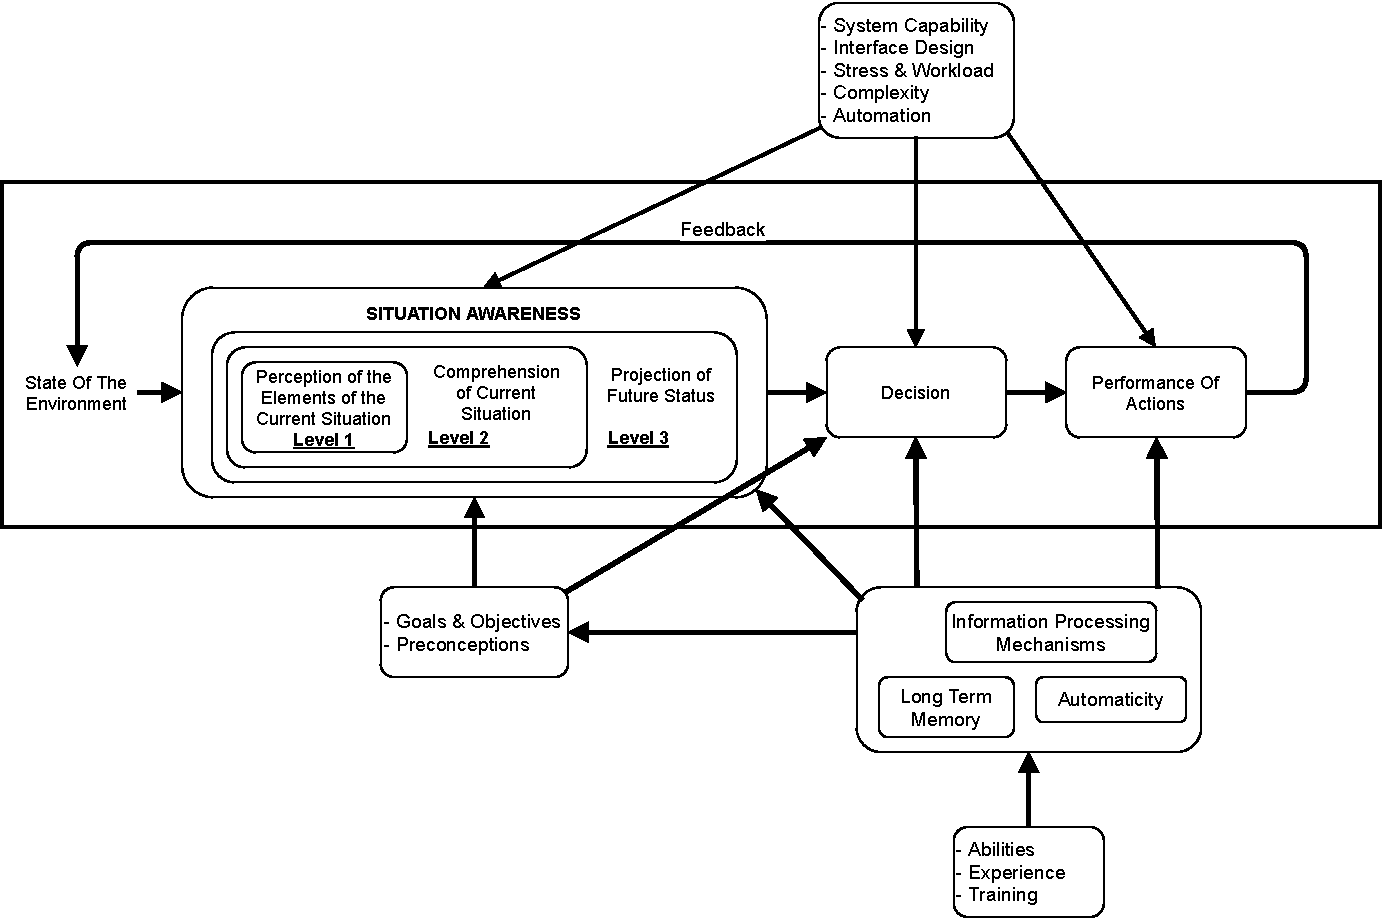
\includegraphics[width=\textwidth]{figures/chap-3/Endsley-1995.pdf}
    \caption{Adapted situational awareness model from \textcite{endsleyTheorySituationAwareness1995}.}
    \label{information:SA}
\end{figure}

% TODO Finir les examples de SA
La définition de la SA précédente a connu de nombreux développements dans l'informatique de crise.

\textcite{fertierRealtimeDataExploitation2020} pour les sytèmes d'instanciation de modèles de situation de crise
Benaben pour les modèles de situations de crise
\textcite{viewegSituationalAwarenessMass2012} la traduit à l'aide d'un coding scheme pour les données issues des médias sociaux
\textcite{vermaNaturalLanguageProcessing2011} propose d'automatiser le traitement des médias sociaux

Numerous works in crisis informatics have extended this definition to meet the needs of this domain.
thus uses the definition of \textcite{endsleyTheorySituationAwareness1995} in that it tries to identify if the content of microblog contents can be useful during massive emergencies.
The author therefore starts from a corpus of messages posted on Twitter during different events and identifies tweets that have the potential to improve situational awareness.

Later, proposed to automate the processing of this information by natural language processing systems.
Inspired by this proposition, several research teams built software to reproduce the results of using computational automation.
These systems aim to improve the user's situational awareness during mass emergencies.
Many systems have been developed to classify tweets \parencite{carageaClassifyingTextMessages2011, imranAIDRArtificialIntelligence2014,ashktorabTweedrMiningTwitter2014}.
More recently, systems proposing a multi-modal approach (image + text) have been proposed.
The multiplication of heterogeneous data collection channels is a promising approach.
This approach enables systems to bring different points of view on the same event to the user.
It also brings an interesting research perspective, especially when merging the two types of data.
The combination of heterogeneous data sources can provide opportunities:

\begin{enumerate}
    \item Collect more information,
    \item Verify certain information when text and image overlap, and
    \item Fill gaps in one information source with that of another.
\end{enumerate}

\subsubsection{Actionable information}
% TODO 
Interviews conducted with crisis managers and operators of call centers revealed that situational awareness was not the only information need expressed by practitioners
\parencite{zadeSituationalAwarenessActionability2018, kropczynskiIdentifyingActionableInformation2018}.
Depending on the nature of the incident, a crisis management team can find themselves lacking
the critical information to take action, or on the contrary, be overloaded with information.
This leads to a situation of paralysis of the decision-makers, despite the fact that they have the necessary information.
The interviewees, therefore, refer to actionable information, i.e., information that enables direct decision-making leading to a physical response.
Thus, as systems that process social media data act as an additional source of information, they can fuel information overload.
Hence, the proper design of these systems is of utmost importance (see Chapter 5).
The rest of this section focuses on this concept, its definition and what it implies for the processing of social media data.

Actionable information can then be considered as a specific type of information.
\textcite{yangDesignPrinciplesIntegrated2012} indicate that the fire response system they propose should focus on information that is (i) timely, (ii) accurate, and (iii) complete.
For instance, information that provide the exact location of the event (accurate information) and the environmental conditions (complete information).
\textcite{comesBringingStructureDisaster2015} call for a similar set of attributes to define the information needed in an information system for crisis response: (i) relevant, (ii) accurate, (iii) timely.
\textcite{zadeSituationalAwarenessActionability2018} conducted a survey and various interviews of emergency and humanitarian responders.
They focused their research on the question "how can the right information reach the right person at the right time?"
In their approach to this research, they first asked practitioners to define actionability.
They report:
\blockquote{"participants described actionable information as anything which either they or their organization could use at that moment to assist, enact, or expedite the solution to a (potentially) identified issue."}
More importantly, the authors report that the practitioners use a different definition depending on their organizational role and responsabilities.
\citeauthor{zadeSituationalAwarenessActionability2018} identified the same attributes as the previous authors.
However, they also highlight the dependence of the definition of actionable information on the role of the receiver of the information.
Thus, information may lead a certain type of decision-maker to actually make a decision, while a decision-maker in charge of another scope may judge the information provided as unimportant.
For instance, an information can be actionable for firefighters, but not for EMS.
The same authors also add a criteria of credibility.
An information that is not convincing will not lead to any response from the decision-makers.
As a result of all the point of views presented, an information is actionable if it is:

\begin{itemize}
    \item Accurate: contains a location
    \item Addressed to the right role: the right decision-maker receives the information
    \item Timely: it reaches the decision-maker at the right time, e.g., avoiding a danger.
    \item Credible: it is taken into account
    \item Complete: it provides sufficient context on the environment.
\end{itemize}

% TODO Check
Each W asked effectively match the actionable information criteria proposed above.
The \textit{Where} question is especially salient, and was mentioned as the most important question.
It is indeed the piece of information that dispatchers will then use to send resources at the location of the event.
All the other questions provide additional context.


% TODO Move to findings
Later, \textcite{kropczynskiRefiningCodingScheme2019} refined the coding scheme was the coding scheme defined in \textcite{kropczynskiIdentifyingActionableInformation2018} with subcategories.
They conducted an analysis of a corpus of tweets to determine how actionable information appears within actual social media posts during a crisis.
At the light of this refined scheme, they coded 200 tweets and reported the proportion of tweets that were fitting in these categories.
Their results show that among the tweets, four of the categories (Where, What, Who, Why) were significantly present, while two (Weapon and When) were rare.
With social media content, the Six W's might process is then slightly modified.
Usually, there is no follow up information to fill the missing attributes like in a regular phone call.
A social media processing therefore have to consider that specificity.
It can be address by aggregating the pieces of information retrieved from both call-takers and social media operators within a unified system.

\subsection{Information needs of a crisis management organization}
La section précédente c'est intéressée aux questions:
\begin{itemize}
    \item What information do decision-makers need?
    \item What information are the operators looking to retrieve?
\end{itemize}

Cette section est alimentée par les findings des interviews et les findings de la littérature.
Cette section vise à réponse à la question initialement posée dans cette partie:
Quelle informations les gens cherchent sur les médias sociaux ?

les informations qui alimentent la situational awareness
On s'appuie sur les 6W's utilisés dans les centres d'appels
Les informations actionables

% ? Rob on the 911 PSAP
The conclusion of \textcite{graceRolePlayingNext2019} highlights some points from the observations,
with the intent to facilitate the construction of future social media processing systems.
\begin{itemize}
    \item The current system lacks flexibility. The operators reported "breakdowns" in the
          information pipeline - corresponding to calls that do not provide the expected information
          or reported elements not relevant with an emergency.
    \item Six W's and ProQA serve as interpretive frameworks during sensemaking processes.
          The authors therefore note that similar systems built to process social media should
          be built with that idea in mind and "for example, pre-filtering and visualizing social
          media data in ways that align with domain-dependent information requirements"
    \item The way information is processed ("the information processing protocol" as per the authors)
          is also important, and in that sense future, social media analysts should receive the
          call-taker's training to create a protocol as similar as possible to theirs, allowing
          a better fluancy between the two information processing pipeline.
\end{itemize}
Also, in this situation, it would not make sense to build a system that is dissociated with the CAD system.
Social media processing has to be integrated into the CAD system the same way as ProQA, using its plugin system.


Specifically, \textcite{jacksonInformationSharingEmergency2006} present four types of information that support situational awareness to protect emergency responders.
These four types of information are:

\begin{enumerate}
    \item Information about the hazard environment
    \item Information on the responder workforce
    \item Information on evolving safety issues
    \item Information about safety equipment
\end{enumerate}

These points are reused later by \textcite{yangDesignPrinciplesIntegrated2012}, that generalized these points, and, more anecdotally, correspond to information that was requested by the decision-makers during the exercises I observed.
This information allows decision-makers to make crisis response decisions while protecting their teams.
These four needs can also be generalized, as discussed at the end of the next sub-section.

Improving situational awareness is a common goal of many social media data aggregation systems and are espoused to address information needs first responders.
Much progress has been made on data aggregation, processing, and analysis thanks to the work of these teams.
However, given that these systems are not often utilized by practitioners, we believe that enhanced situational awareness alone is unsatisfactory.
Instead, evidence pointing to the need to consider other aspects of the information processing pipeline bears consideration in the development of new data systems.

% TODO Rajouter Yang
The information needs of decision-makers depend on the crisis at hand.
However, from the results of the above-mentioned observations, one can identify patterns that would be common in most of the situations faced and that are crucial to the decision-making process.
The decision-makers express several needs.
First, they need constant and specific information (what is the emergency? where is the emergency? etc.)
This information is obvious for crisis management and as such, is barely mentioned in the interviews, which are often oriented towards identifying less visible needs.
The information sought through the Six W's and the information needed exposed by \textcite{jacksonInformationSharingEmergency2006} compose what would be the "baseline" information needs.
These are:

\begin{enumerate}
    \item Location of event, type, cause and severity;
    \item Environmental conditions (buildings, population density, potential hazards and their location, etc.);
    \item Information on the response participants (responders already involved, their skills, resources, etc.);
    \item Current and future needs of the responders (number of casualties, their status, etc.); and
    \item The available resources to the event (qualified actors, appropriate equipment, etc.)
\end{enumerate}

In addition to these basic information needs, when asked, emergency management organizations request "actionable information".
An actionable information is a piece, or the last missing piece, of information which enables immediate decision-making.
Actionable information can be seen as a "super information", i.e., an information with additional properties.
It is an information that:

\begin{itemize}
    \item is located;
    \item is directed to the right role;
    \item is timely;
    \item is credible;
    \item provides context.
\end{itemize}

The different attributes are ordered by importance.
A response can be triggered if the decision-maker (or the dispatcher) can understand the emergency
and know where to allocate resources.
But crisis management often involvs multiple, distributed actors that are not necessarily
used to work together.
Thus, it is not uncommon for one of the actors to have information that is of little interest to him,
but which turns out to be critical for another actor.
The timing of this information is important, as information that arrives too late can be rendered useless.
Having information coming from a trustworthy source is also an advantage.
The crisis managers I met with and asked about credibility said that in the case of a message
mentioning an emergency and whose source is not trustworthy, they send a team to recon.
During the first exercise of the MACIV project,  social media messages sent by ordinary
citizens and whose veracity they could not confirm were processed this way by the emergency managers.
The "additional context" criteria correspond to the other pieces of information required
by decision-makers to respond effectively to the event.
While credibility, context and the mention of a location of information are properties of the information, the criteria of "right person at the right time" criteria are more linked
to the organization in charge of the response.

In this view, actionable information is information that matches several criteria that would lead a decision-maker to make a decision and send resources.
Actionable information is the trigger of the resource allocation.
However, proper response that would lead to the resolution of the event requires additional information.
It is information that is latent to the situation (hazards, deployed and available resources, victims, etc.).
These additional pieces of information are part of the "context" of the crisis (resources available, responders already deployed, etc.).
This information constitutes, as explained above, the decision-maker's situational awareness.

% TODO Inclure dans le texte
Figure~\ref{information:sa-inf} summarizes the link between situational awareness and actionable information.

% TODO Cropper 
\begin{figure}[htb]
    \centering
    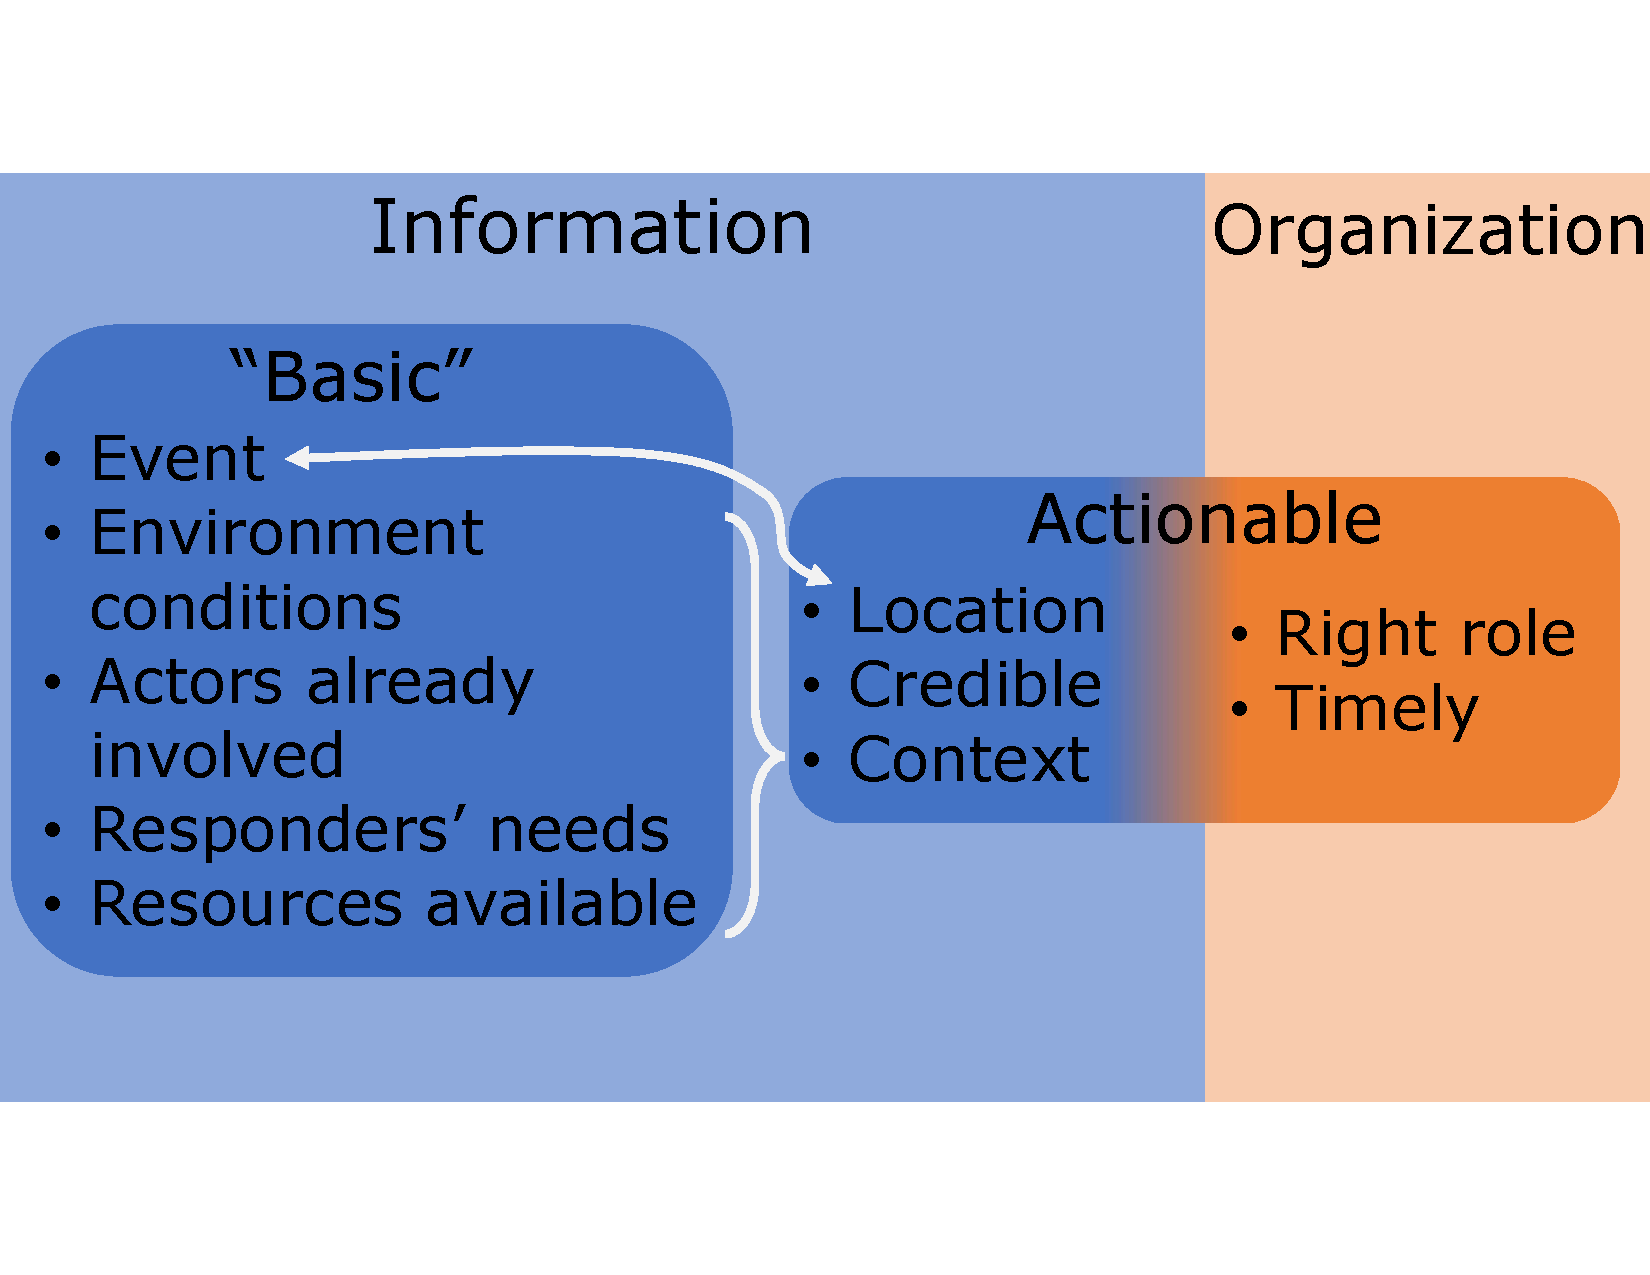
\includegraphics[width=\textwidth]{figures/chap-3/sa-ainf.pdf}
    \caption{Shared attributes between elemental information needs for crisis response and criteria for an information to be actionable.}
    \label{information:sa-inf}
\end{figure}

\subsection{Location of actionable information in the situational awareness model}
Situational awareness is the initial building block of decision-making in crisis response.
Information cannot be designated as actionable without the decision-maker having sufficient context to decide if that information is actionable.
Therefore, crisis management starts by recovering an adequate perception of the elements/assets of the environment (level 1 of SA).
From that perception, they will use their skills/training to understand (level 2 of SA) the current situation.
Then, decision-makers evaluate the future status of their environment (level 3 of SA).
In this picture, an actionable information is information that can immediately triggers a decision from the decision-makers.
For instance, a social media operator receives a report of an injured person.
The decisions makers would need to know the location of the victim and which type of equipment is required.
However, if they don't know the status of their evacuation resources or a safe zone to evacuate,
due to the disruption created by the event, they might prefer to not consider this piece of information as actionable.
While it is a useful and important piece of information, decision-makers have to delay their final decision on the evacuation.
In this case, they would prefer to recover a better situation awareness.
Only when they will have a sufficient perception of their environment they will be able to order the evacuation of the injured person.

% TODO Mettre la version enrichit de ce framework
Both the concept of Actionable Information and Situational Awareness are then linked to the concept of Information.
Here, we use the definitions of Data and Information proposed by \textcite{ackoffDataWisdom1989} in his Data-Information-Knowledge-Wisdom framework.
The concept of Data is an abstraction.
It refers to symbols that have no meaning beyond their existence.
Information on the other hand, is data that has been given meaning by the creation of connections between those points.
Information generally answers questions such as "who," "what," "where" and "when."
Thus, the caller takers interviewed in \textcite{kropczynskiIdentifyingActionableInformation2018} are gathering Information through the Six W's.

Information and Data are also present in the Situational Awareness model proposed in \textcite{endsleyTheorySituationAwareness1995}.
To the three levels proposed, and described earlier in the literature review, we can associate the Data-Information-Knowledge concepts as proposed in Figure~\ref{information:SA-DIK}.

\begin{figure}[htb]
    \centering
    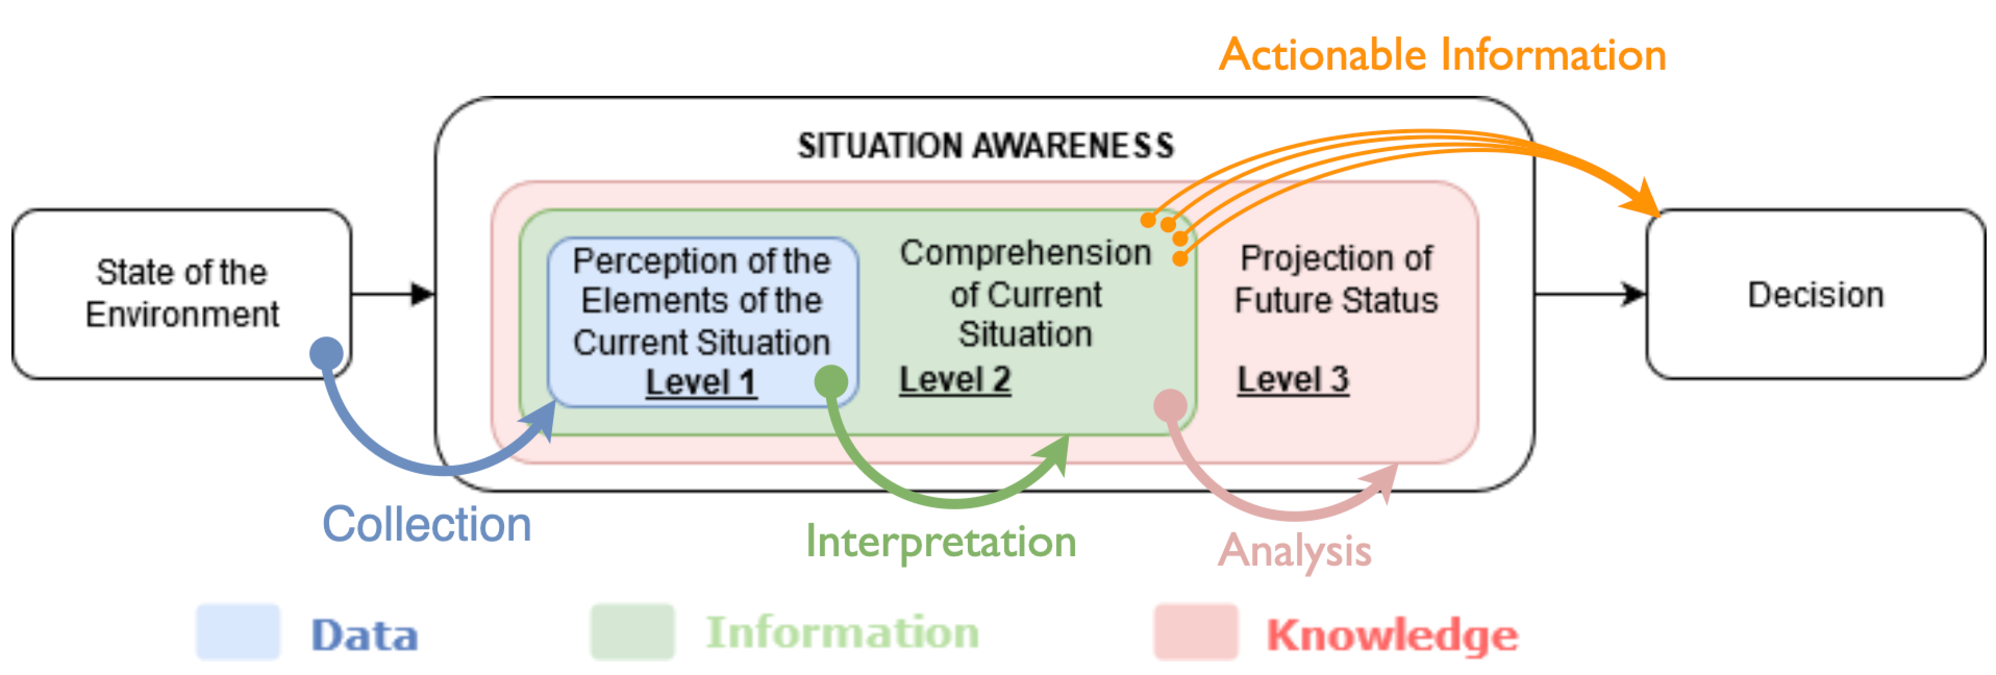
\includegraphics[width=\textwidth]{figures/chap-3/Fig2-2.pdf}
    \caption{Location of Data-Information-Knowledge concepts in the Situational Awareness model}
    \label{information:SA-DIK}
\end{figure}

The first level of Situational Awareness concerns the perception of the "elements/assets" (or data) of the environment.
Effective data collection allows a decision-maker to achieve a sufficient perception of the surrounding environment and a means to describe it.
Assuming this first level is effective, the second level of Situational Awareness consists of being able to form patterns with the other elements/assets.
Through the interpretation of the different data points and the way they interact with each other, the operator is able to understand the ongoing situation.
This is this level of Situational Awareness that decision-makers are required to reach to be able to make decision.
This is also this same level that is often lost during the chaotic nature of a mass emergency event, and that decision-makers try to recover using situational awareness tools \parencite{endsleyTheorySituationAwareness1995}.
The final level uses the patterns known or identified by the decision-makers to make predictions on the future states of the environment, thus referring to the Knowledge layer of the framework.
It is preferred that the decision-maker has this level of Situational Awareness, but it is not necessarily required.

Situational Awareness is built upon any Data or Information about the current state of an environment, and that is delivered to the decision-maker.
Using the previous proposition, we are now able to envision a relationship between Situational Awareness and Actionable Information.
As Actionable Information is a type of Information, it is then embedded in the second level of Situational Awareness.
The difference with regular Information is that Actionable Information is the missing piece of the puzzle that allows the decision-makers to decide.
As a result, Situational Awareness is the puzzle comprised of pieces of Information that
decision-makers try to assemble during the event, and Actionable Information constitutes
the final, missing pieces of that puzzle necessary to comprehend the whole.
Actionable Information is then a specific piece of Information in the Situational Awareness model.

All these criteria are context dependent.
As an example, when is information delivered "at the right time"?
The right time can be seen as a time window allowed by the acquisition of previous incomplete
information, with missing parts and where a new incoming information complete the puzzle.
Timeliness, credibility and adequacy of the role, as subjective criteria, are mostly context dependent.
It is therefore very difficult to set a threshold for these values that would "simply" collect Actionable Information.
\textcite{silberschatzWhatMakesPatterns1996} describe two major issues with the processing of Actionable Information:
(i) there are a lot of patterns of interest, that have to be divided into a finite set of action-pattern equivalence;
(ii) pattern-action associations are likely to change overtime, thus, the life cycle of these associations has to be managed.
The concept of actionable information is important, yet and fuzzy and context-dependant, as the criteria above show.

% TODO Supprimer le summary
\subsection*{Summary}
This section sought to answer two questions:
\begin{itemize}
    \item What information do decision-makers need?
    \item What information are the operators looking to retrieve?
\end{itemize}
Call-takers and social media operators are looking for information that meets minimal requirements.
However, information that meets one of these requirements, provides a location and that is delivered
to the right person, at the right time, is described as an actionable information.
Actionable information is requested by crisis management organizations, as they are information that
facilitate decision-making and therefore provide greater results.
In real world situation, it is very challenging and rare to have information that corresponds to all criteria simultaneously.
Social media, as others information channel cannot provide alone actionable information.
On the other hand, social media can provide pieces of information that improve the situation
awareness of the decision-makers by adding elements to the context.
This additional context can then, on some occasions, provide actionable information.
However, this capacity can only be unlocked by creating a direct and collaborative means
of communication between the operators responsible for monitoring the different information channels.
This information system calls for an ontology, or information model, that is able to take
into account information from both channels.
The aim of the next section is to define this abstraction in the light of the elements
presented so far.

\section{Information expected by information systems}
% TODO when you expect the output of the social science study to inform, and serve as input to your model is weak
% TODO 3.4, 3.4.1 and 3.4.2 needs to be much more clear.
% TODO Exactly what is the output from the first phase.
% TODO Exactly what is the input to the model.
% TODO How will this be automated?
% TODO How will this remain valid and true to the real world?
% ? La première partie de ce chapitre a présentée le besoin en information des organisations en charge de la réponse et de ses différents acteurs
% ? La prochaine section présente ce besoin du point de vue d'un système d'information
% ? C'est à dire: quelles données/informations sont nécessaires au fonctionnement d'un SI ?

% TODO Ajouter ISYCRI (ou je sais psa quoi de 2006)
As presented in the first chapter, the crisis response phase requires the deployment of resources that are very quickly stretched.
Moreover, an adequate and efficient response cannot be put in place without prior information.
The automation of the collection and support of information processing is therefore a considerable advantage in a crisis situation.
However, such a capability requires an information model capable of representing the information that responders need \parencite{comesBringingStructureDisaster2015}.
The first sub-section attempts to integrate actionable information into the model used to describe situational awareness.
The objective of this sub-section is to consider how the notion of actionable information can support the construction of an information model for crisis response.
The second sub-section presents an information model for the response.

\subsection{Information managed by existing crisis situation models}
% TODO Préciser pourquoi les modèles d'information sont important.
\label{sec:crisismetamodel}
Le chapitre precedent a dresse un historique des modeles d'information développés pour la gestion de crise (section\hyperref[sec:lit-information-models]{2.2.1}).
Ces modèles permettent de représenter informatiquement l
Deux modèles émergent dans le cadre de l'amélioration de la collaboration entre différents acteurs de la gestion de crise \parencite{othmanDevelopmentValidationDisaster2014,benabenMetamodelItsOntology2008}.
\textcite{othmanDevelopmentValidationDisaster2014} propose metamodels for disaster management.
Hence, they created a metamodel for each phase of crisis management they consider: mitigation, preparation, response and recovery.
Their proposition is represented Figure~\ref{information:othman-metamodel}.
Their model is consituted of four principles entities: \textbf{Disaster}, \textbf{Rescue}, \textbf{EmergencyManagementTeam}, \textbf{ResponseOrganization}, and \textbf{EmergencyOperationCentre}.
The latter is a \textbf{ResponseOrganization} that controls the \textbf{EmergencyManagementTeam}.
A \textbf{ResponseOrganization} uses \textit{Aids} and \textit{Resources} at its disposal and is organized according to an \textit{EmergencyPlan}.
It supports the \textbf{Rescue} teams in their efforts to rescue \textit{Victims} according to their \textit{Situational Awareness} and their \textit{Exposure} to the \textbf{Disaster}.
The \textbf{Rescue} teams are managed by a \textbf{EmergencyManagementTeam}.
This team is in charge of defining a set of \textit{ResponseTask} according to some \textit{ResponseGoal}.
It follows \textit{Command}, requires \textit{Coordination} and uses means of \textit{Communication}.

\begin{figure}[htb]
    \centering
    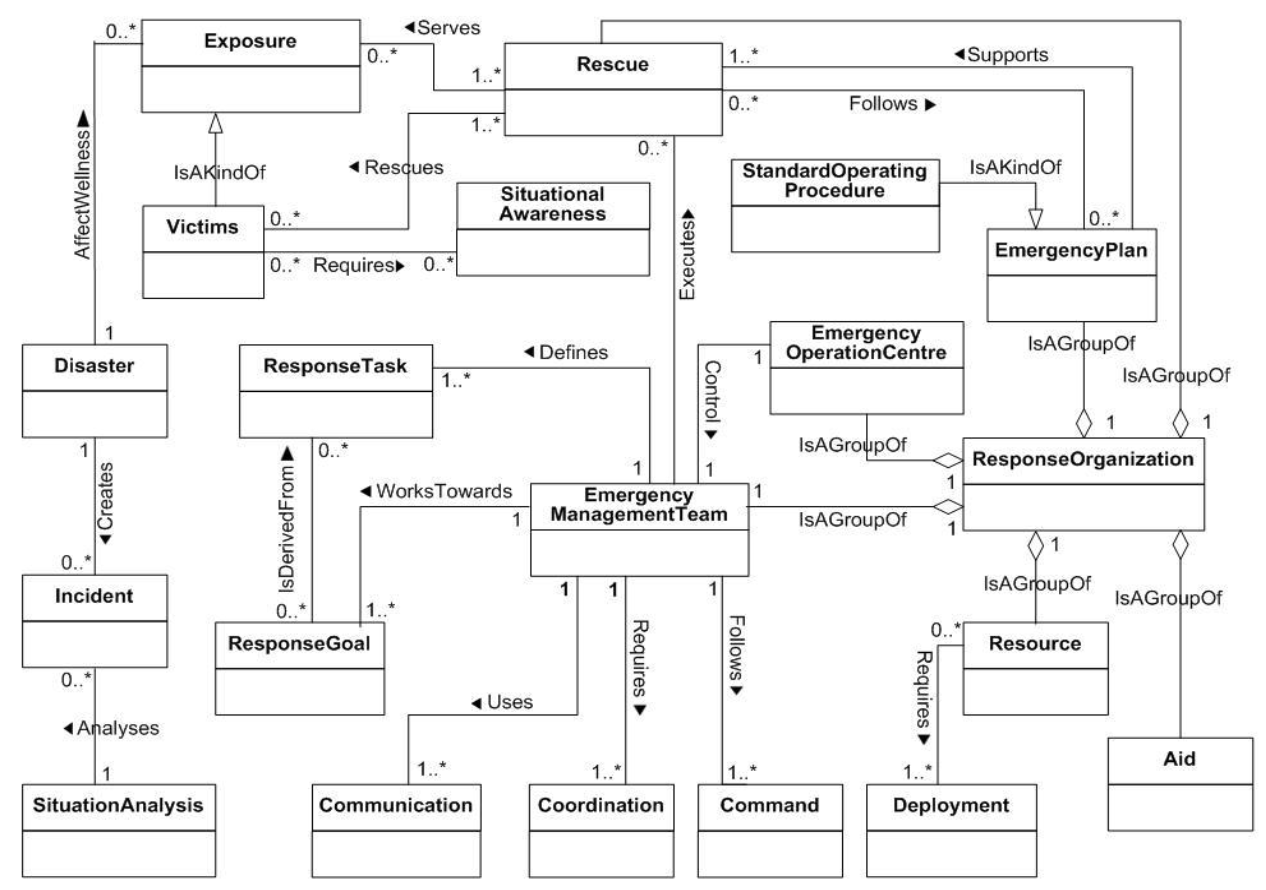
\includegraphics[width=\textwidth]{figures/chap-3/othman-metamodel-response.PNG}
    \caption{Metamodel proposed by \textcite[Fig.4]{othmanDevelopmentValidationDisaster2014} for the response phase of a disaster event.}
    \label{information:othman-metamodel}
\end{figure}

On the other hand, the metamodel proposed by \textcite{benabenMetamodelKnowledgeManagement2016} focuses on the collaboration during the response phase.
This metamodel is split in five packages: \textbf{Core}, \textbf{Partners}, \textbf{Context}, \textbf{Objectives} and \textbf{Behavior}.
Figure~\ref{information:benaben-metamodel} represents the four main packages: \textbf{Core}, \textbf{Partners}, \textbf{Context} and \textbf{Objectives}.
The \textbf{Behavior} package is excluded as it is solely used to implement a process model of the collaborative behavior using the Business Process Model and Notation (BPMN) representation.

The \textbf{Core} package describes the collaborative process.
This package is composed of five sub-systems: the \textit{Context} system, the \textit{Objectives} system, the \textit{Partner} system, the \textit{Performance} system and the \textit{Behavior} system.
Each system represent a certain aspect of a collaboration.
The collaboration happens in a given \textit{Context} that contains \textit{Characteristics} and \textit{Threat/Opportunities}.
\textit{Partners} collaborate in this \textit{Context} according to their \text{Resources} and \text{Capacities} in response to an \text{Event}.
The different \textit{Partners} collaborate towards \textit{Objectives}.
During their collaboration, they review their \textit{Performance} in achieving their \textit{Objectives}.
This package is generic to any collaborative endeavour.
Thus, the metamodel is specified to crisis situations through the surrounding packages.

\begin{figure}[htb]
    \centering
    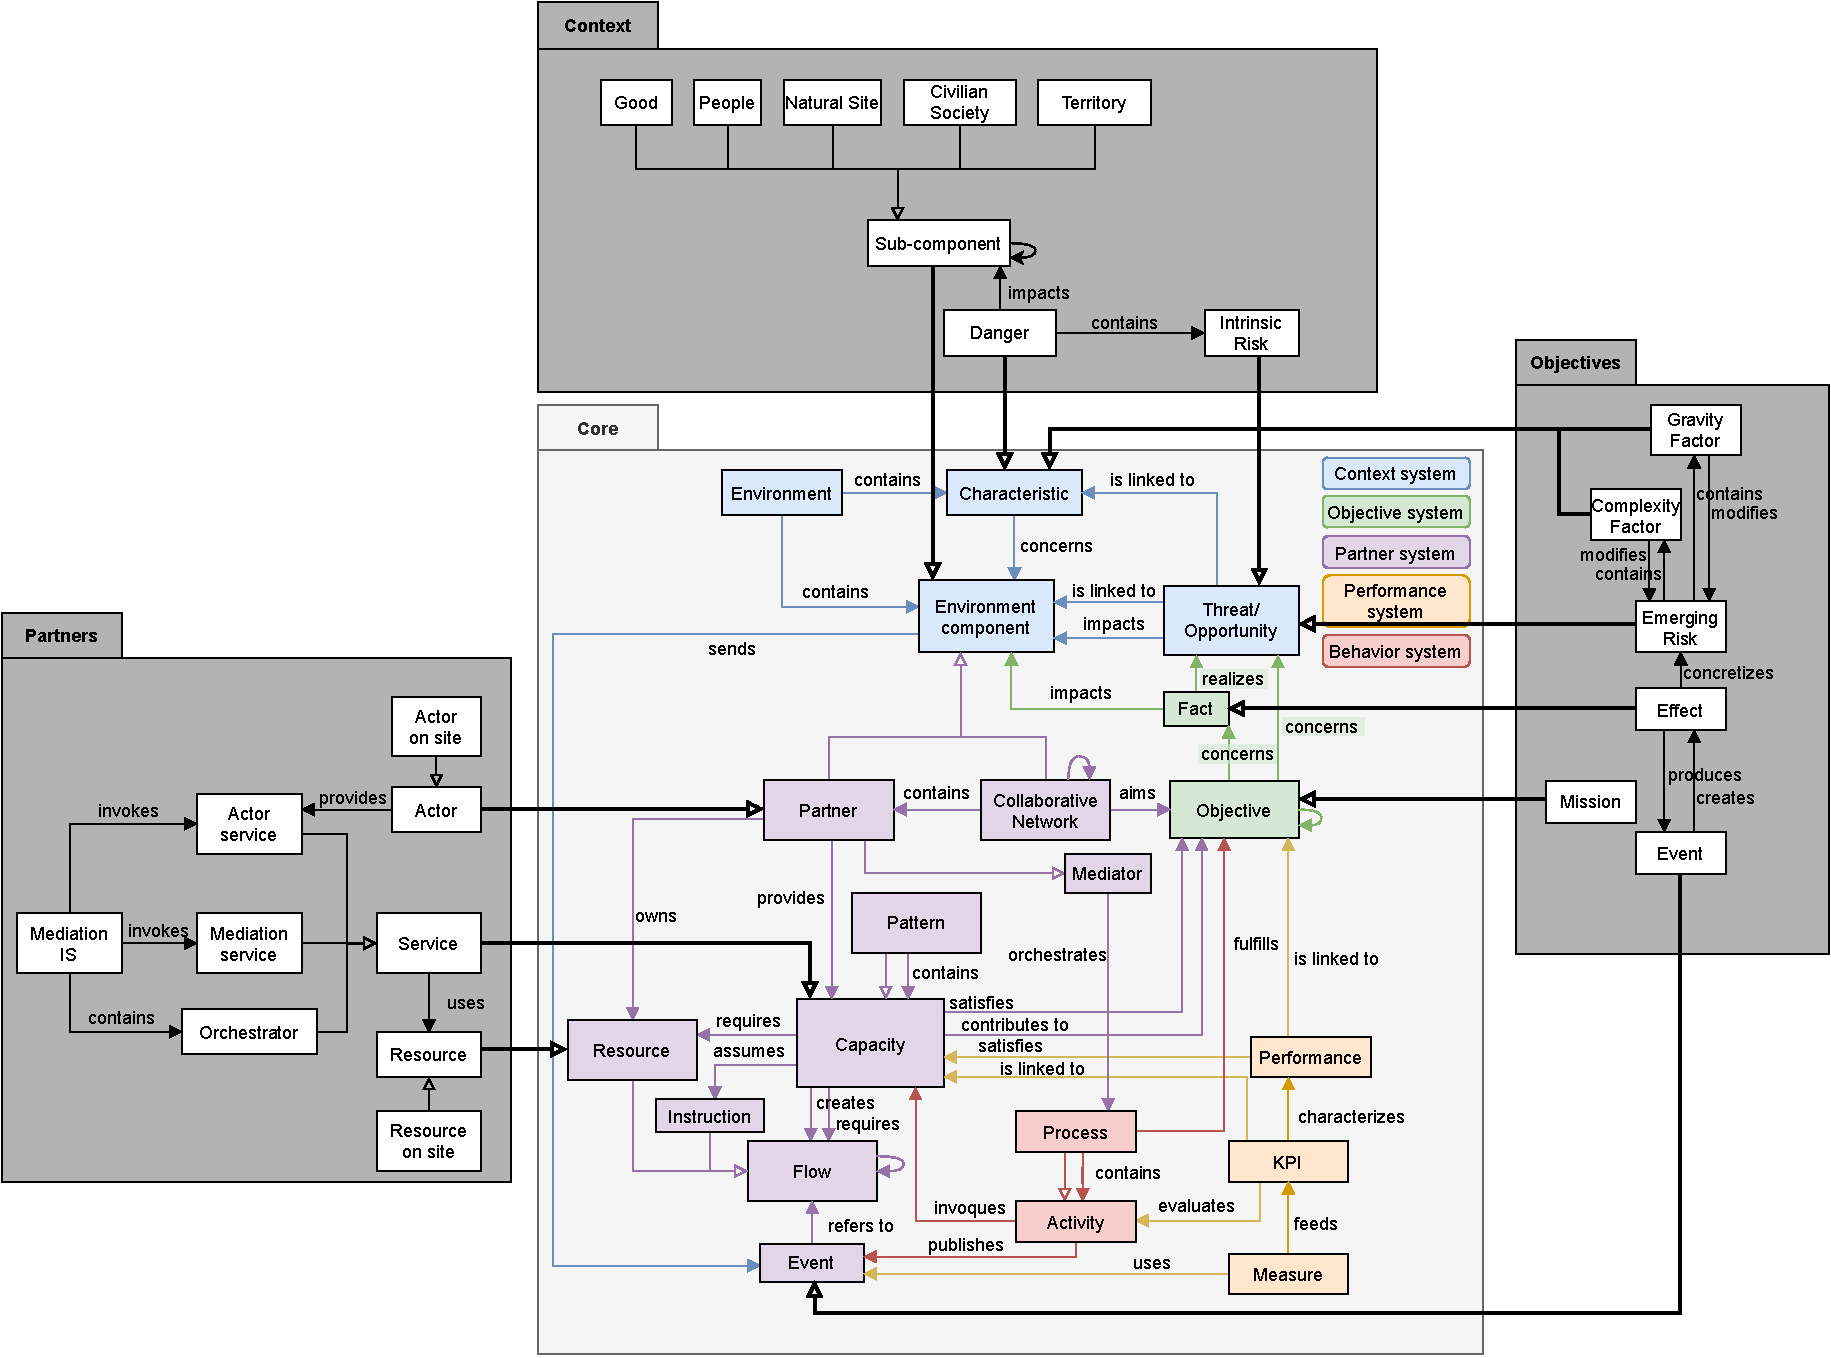
\includegraphics[width=\textwidth]{figures/chap-3/benaben-metamodel-response.pdf}
    \caption{Metamodel proposed by \textcite{benabenMetamodelKnowledgeManagement2016} for the response phase of a disaster event.}
    \label{information:benaben-metamodel}
\end{figure}

The Context package provides additional classes to represent the disaster environment.
It is composed of:
\begin{itemize}
    \item \textit{Good}: human-made elements such as roads, buildings, etc.
    \item \textit{People}: group of persons
    \item \textit{Natural site}: natural elements such as forest, lake, etc.
    \item \textit{Civilian society}: social actors such as media, institution, etc.
    \item \textit{Territory}: administrative area such as county, region, etc.
    \item \textit{Danger}: dangerous characteristics linked to the context such as seismic area, social instabilities, etc.
    \item \textit{Intrinsik risk}: risk linked to the previous dangers identified which, in the previous example, would correspond to earthquake and riots.
\end{itemize}

The Partners package contains:
\begin{itemize}
    \item \textit{Actor}: emergency responders such as firemen, EMS, etc.
    \item \textit{Resource}: resource used by actors such as, a truck, an ambulance for the previous actors
    \item \textit{Service}: capabilities of actors, which correspond to evacuate people and treat injured ones.
    \item \textit{Actor service}: service specifically provided by actors.
    \item \textit{Mediation service}: services provided by the information system used by the partners.
\end{itemize}

The Objectives package:
\begin{itemize}
    \item \textit{Emerging risk}: risk resulting from the event itself (e.g. collapse of a building, panic, etc.).
    \item \textit{Effect}: direct consequence of the crisis itself (e.g. 10 injured people, fire, etc.).
    \item \textit{Mission}: objective directly linked to identified risk or effect.
    \item \textit{Event}: event occurring during crisis management that must be considered as triggering an effect.
    \item \textit{Gravity factor}: characteristic of the current situation that may increase or decrease the gravity of the crisis (e.g. rain or wind on a large fire).
    \item \textit{Complexity factor}: characteristic of the current situation that may change the type of the crisis.
\end{itemize}

Si les deux metamodeles visent tous les deux à représenter la collaboration entre les différents acteurs de la réponse, les deux modeles different par leurs approches.
On the one hand, the metamodel proposed by \textcite{othmanDevelopmentValidationDisaster2014} est un modèle qui s'inscrit dans une modélisation complète de la gestion de crise.
De plus, s'axe principalement sur la description de la collaboration entre les différents acteurs.
De plus, on remarque que certaines entitées identifiées dans le chapitre précédent sont ne sont ou insuffisament décrites.
Notament, la description de l'envrionnement, attendu par les acteurs de la reponse, est décrit uniquement au travers de la classe Exposure.
De la même manière, l'événement apparait essentiellement au travers de la classe Disaster.
Le modèle proposé par le \textcite{othmanDevelopmentValidationDisaster2014} permet donc de décrire efficacement la collaboration entre les acteurs de la crise.
Cependant, il décrit insuffisament la collaboration, dans le contexte de la crise.
On the other hand, \textcite{benabenMetamodelKnowledgeManagement2016} dedicated packages allow for a more precise description of key concepts for the Situation Awareness and Actionable Information.
% TODO Faire l'union des deux modèles.
% TODO Conclure et lier à la suite 

\section{Actionable information for decision makers that can be processed automatically}
As \textcite{zadeSituationalAwarenessActionability2018} highlighted, proposed social media systems have not been widely adopted by emergency responders.
Among all the reasons that could explain this lack of interest, some are certainly related to the design of the systems.
Systems initially developed were focused on increasing the amount of information provided to first responders.
However, the misfit of the categories used by these classification systems ultimately lead to adding noise in the processing.
In addition, the information did not always fit the responder's need, resulting in additional noise.
Current systems handle data collection and information extraction.
But the resulting flow might still be overwhelming for social media operators.
The systems developed should require a minimal amount of attention from the operators on the menial tasks, while keeping her engaged.
As the goal of increasing the volume of information available to emergency managers can be considered as achieved, future work could concern information quality.
This quality improvement can be achieved by adding support to Actionable Information identification.
But, as stated earlier, Actionable Information can be identified by systems only by having a sufficient Situational Awareness at first hand.
Thus, social media processing systems need to be able to both perceive and comprehend the situation.
Also, initially difficult to focus an information system on the concept of Actionable Information,
because it is very challenging to define clearly "the right person at the right time."
The criteria of location, contextualization, and credibility of the information already offer more opportunities from an information system perspective.
An information system to support social media operators in crisis response is therefore more centered around situational awareness.
Thus, it considers the two types of actors that interact with the model.
The model must meet the needs of both actors and, in particular, not hinder their workflow.
Call-takers must be able to submit the information they consider relevant.
Decision-makers must be able to quickly identify the information they need during the response.

All these considerations lead to the information model summarized in Figure~\ref{information:information-models}.
A more complete version described using the UML 2.0 specification can be found Appendix A.

\begin{figure}[htb]
    \centering
    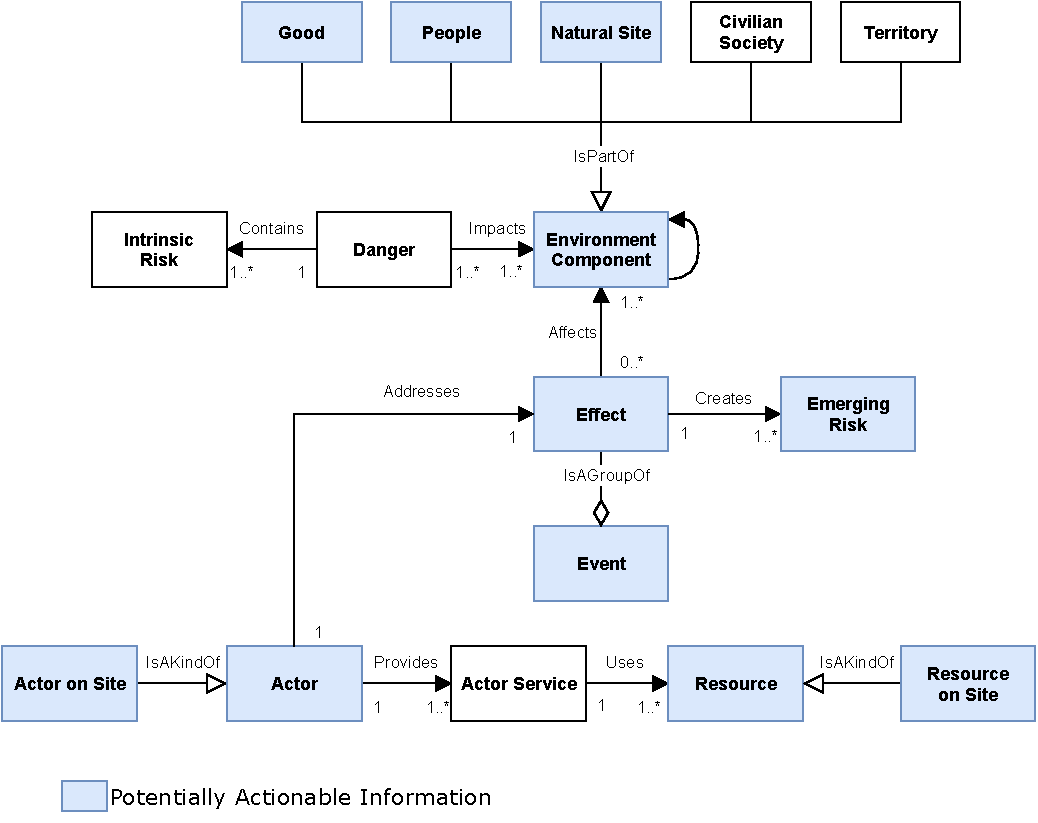
\includegraphics[width=\textwidth]{figures/chap-3/information-needs.pdf}
    \caption{Proposed information model, produced after reviewing the information handled the call-takers and needed by decision-makers.}
    \label{information:information-models}
\end{figure}

The model is composed of nine entities:
\begin{itemize}
    \item Event
    \item Environment
    \item Actors involved
    \item Responders needs
    \item Resources available
    \item Location
    \item Hazard
    \item Equipment
    \item Actors
\end{itemize}

% TODO Mettre en avant les entités du modèle dans la suite des explications.
It is centered around the concept of Event.
Several attributes allow the call-takers/social media operators to describe an event such as
the Location, the type, the severity, or the cause.
The Location of an event can be a specific address, the name of a place or a generic one,
such as a neighborhood, an indication of a city blocks, etc.
The Event entity is linked to four other entities that are responsible for informing the event.
These entities are Environment, Actors involved, Responders needs and Resources available.

An Event takes place in an Environment.
An environment can have a population density, hazards or indications provided by the callers.
There may also be different types of hazards, which may or may not be localized.
An environment can host several events, possess multiple hazards, see multiple actors involved
that have different needs.
Hence, entities that describe who are involved in an event (Actors involved) that describe the
Actors involved and their Equipment.
The actors have different skills, like firemen or policemen in the case of professionals.
However, there may also be civilian actors who may or may not have skills.
A similar reasoning is applied to Equipment, which are often used in the fight against specific hazards.
The Actors involved have (or are going to have needs) according to the type of event and the
specificities of the environment.
In order to fight an event and address hazards, responders have access to Resources Available.
The resources are composed of actors or equipments that are not engaged in an action.

The proposed information model is reused throughout the rest of the manuscript.
Chapter 4 presents an algorithm that aims at automatically detecting previous entities in messages.
Chapter 5 proposes an architecture for the above-mentioned information system, which is built around the entities described in this chapter.

\section*{Conclusion}
This chapter explored the information needs of decision-makers during crisis response and
proposes an information model to build an information system to support crisis management organizations.
The needs retained are:

\begin{enumerate}
    \item Event (location, type, cause and severity);
    \item Environmental conditions (buildings, population density, potential hazards and their location, etc.);
    \item Information on the response participants (responders already involved, their skills, resources, etc.);
    \item Current and future needs of the responders (number of casualties, their status, etc.); and
    \item Resources available for the response (qualified actors, appropriate equipment, etc.)
\end{enumerate}

This chapter discussed two concepts widely used in the crisis management community: situational awareness and actionable information.
\textcite{zadeSituationalAwarenessActionability2018} proposed that actionable information is information that trigger immediate response.
We have taken the definition of these two concepts and developed how they can be adapted to the content available on social media.
In particular, we have seen that in practice, response teams are primarily looking for actionable information.
However, the individual data available on social media very rarely meets all the criteria that would allow them to define their information as actionable.
If relevant information posted on social media is rare, golden tweets are even rarer.
However, if we go back to the concept of situational awareness, we understand that actionable information is not an entity living in a vacuum in the middle of the crisis.
Actionable information is in fact extremely linked to its context and lives only in it.
This underlines the importance, as a decision-maker, of having the best possible overview of the situation, in order to determine
whether a piece of information is actionable, or to which other actor it might be.
For social media operators, in charge of content processing, it is (I think) illusory to find actionable information as it is in social media.
On the contrary, they should expect to find pieces of information that, similar to
similar to puzzle pieces, lead to actionable information once assembled.

As a final note, decision-makers need actionable information to make decisions.
The role of the social media operator is to look for bits and pieces of information, which when aggregated can provide actionable information.
Not all data has to come from social media alone.
As mentioned earlier, \textcite{graceRolePlayingNext2019} emphasize the importance of
maintaining a similar information processing protocol between call-takers and social media
operators, in order to maintain the existing fluidity.
This calls for a tool capable of bridging the gap between the two mediums, based on
abstraction that crosses the information needs of decision-makers and the information that
information that the operators can actually retrieve.The literature review highlighted previous
propositions of ontologies and metamodels, that are, in shape similar to the information model proposed in this chapter.
The proposition made in this chapter differs from the point of view adopted.
Instead of focusing on the system or a particular aspect of crisis management,
the emphasize is set on the information flow between a specific set of actors that are crucial to crisis response.
For instance, \textcite{benabenMetamodelKnowledgeManagement2016} proposed a metamodel of collaboration between crisis actors.
This metamodel models the sharing of information between the different actors, the keystone of the collaboration.
The model proposed is a "zoom" on the information sharing between the decision-makers and the operators in charge of the information acquisition.
The consideration of other metamodels in crisis management is discussed in Chapter 5.

The model thus obtained makes it possible to manipulate the information exchanged by the decision-makers and operators.
decision-makers and operators.
This offers the opportunity to automatically create instances of the model's classes.
However, this requires a method
capable of detecting information in the social media data.
The next chapter therefore proposes a method allowing to extract the required information required while adapting to the particular context of crisis management.

%%% Local Variables:
%%% mode: latex
%%% TeX-master: "../ma-these.tex"
%%% End:
